%!TEX root = ../thesis.tex
%*******************************************************************************
%*********************************** Chapter 1 *********************************
%*******************************************************************************

\chapter{INTRODUCTION}
\label{chap:intro}

\ifpdf
    \graphicspath{{Chapter1/Figs/Raster/}{Chapter1/Figs/PDF/}{Chapter1/Figs/}}
\else
    \graphicspath{{Chapter1/Figs/Vector/}{Chapter1/Figs/}}
\fi

% ------------------------------ Abbreviations ---------------------------------
% The entries below are collected into the "List of Abbreviations" (group Z).
\nomenclature[z-VQA]{VQA}{Visual Question Answering}
\nomenclature[z-VLM]{VLM}{Vision-Language Model: a model that takes both images and text and generates text}
\nomenclature[z-OCR]{OCR}{Optical Character Recognition: recognising the text in an image}
\nomenclature[z-PEFT]{PEFT}{Parameter-Efficient Fine-Tuning: training only a very small fraction of the parameters}
\nomenclature[z-LoRA]{LoRA}{Low-Rank Adaptation: adds two low-rank matrices to linear layers and trains only those}
\nomenclature[z-QLoRA]{QLoRA}{LoRA on a base model quantised to 4 bits (NF4)}
\nomenclature[z-NF4]{NF4}{4-bit NormalFloat: a 4-bit quantisation data type}
\nomenclature[z-EM]{EM}{Exact Match: the answer equals the gold answer after normalisation}
\nomenclature[z-VQA-Acc]{VQA-Acc}{VQA Accuracy: min(number of matching gold answers / 3, 1)}
\nomenclature[z-ANLS]{ANLS}{Average Normalized Levenshtein Similarity: character-level similarity}
\nomenclature[z-POPE]{POPE}{Polling-based Object Probing Evaluation: measures hallucination with yes/no questions}
\nomenclature[z-SOTA]{SOTA}{State of the art: the best published result}

This chapter introduces the thesis, moving from the problem to the proposed solution.
Section~\ref{sec:intro-overview} gives the general information and an overall
picture of the system. Section~\ref{sec:intro-background} presents the background:
visual question answering, the need to read Vietnamese text in images, the
difficulties specific to Vietnamese and the resource constraints.
Section~\ref{sec:intro-problem} states the problem and splits it into
sub-problems. Sections~\ref{sec:intro-gaps} to~\ref{sec:intro-significance} present
the research gaps, objectives, research questions, hypotheses, contributions and
significance of the work. Section~\ref{sec:intro-scope} defines the scope and
limitations. Sections~\ref{sec:intro-team} and~\ref{sec:intro-pm} summarise how the team was organised and how the project was managed; the details are in
Appendix~\ref{appendix:pm}.

%********************************** Section 1.1 ********************************
\section{Overview}
\label{sec:intro-overview}

\subsection{Project information}

\begin{itemize}
  \item \textbf{Title:} Efficient Vietnamese Visual Question Answering using
  Vision-Language Models.
  \item \textbf{Vietnamese title:} \vi{Nghiên cứu hệ thống hỏi đáp trực quan tiếng
  Việt hiệu quả sử dụng mô hình Vision-Language}.
  \item \textbf{Short name:} ViVQA-VLM.
  \item \textbf{Project code:} FA26AI29. \textbf{Team code:} GFA26AI35.
  \item \textbf{Course:} AIP491, graduation thesis in Artificial Intelligence, FPT
  University.
  \item \textbf{Duration:} 15 weeks, from 7 September 2026 to December 2026.
  \item \textbf{Members:}
  \begin{itemize}
    \item Pham Le Huy Hoang (SE182670), team leader, in charge of PEFT / Training;
    \item Ho Dac Toan (SE183249), in charge of VLM / Baseline;
    \item Tran Quoc Huan (SE193642), in charge of Dataset / OCR;
    \item Van Quang Truong (SE182458), in charge of Evaluation / Deployment.
  \end{itemize}
  \item \textbf{Supervisors:} Assoc. Prof. Duc Ngoc Minh Dang and Mr. Tri Minh Pham.
\end{itemize}

\subsection{Project overview}

Taking a photo with a phone has become a common way to look up information: a user
photographs a shop sign, a medicine box or a menu and immediately wants to ask
``what is the name of this shop?'' or ``what is the phone number?''. The problem
behind this need is Visual Question Answering (VQA). Current open-source
vision-language models (VLMs) solve it fairly well in English, but in Vietnamese
they often answer in English, answer at length, lose the diacritics when reading,
or talk about things that are not in the image.

This thesis studies how to adapt an open-source VLM to Vietnamese VQA at low cost:
only a small adapter is trained, the base model is kept frozen, and every
experiment runs on a single Google Colab GPU. The system has four main capabilities:

\begin{itemize}
  \item it answers Vietnamese questions about the general content of an image
  (colour, count, objects, position) with a short answer in the right format;
  \item it reads Vietnamese text with diacritics on shop signs, product labels and
  price boards to answer questions that require reading;
  \item it shows the OCR text read from the image and a confidence level, so that
  users can check the answer themselves;
  \item it runs on one GPU with less than 8.4~GB of memory for training and less
  than 5~GB for the prototype.
\end{itemize}

Figure~\ref{fig:intro-overview} shows the system from the user's point of view. The
input is an image and a Vietnamese question. If the image contains text,
PaddleOCR~\cite{du2020ppocr} detects the text regions and VietOCR~\cite{vietocr}
reads them, keeping the diacritics; this line of text is added to the prompt
together with the image and the question. The base model
Qwen2.5-VL-3B-Instruct~\cite{bai2025qwen25vl} is compressed to 4 bits and frozen;
we train only a LoRA adapter that accounts for 0.196\% of the parameters.
The output is a short Vietnamese answer, with the OCR text as evidence when
available.

\begin{figure}[htbp]
\centering
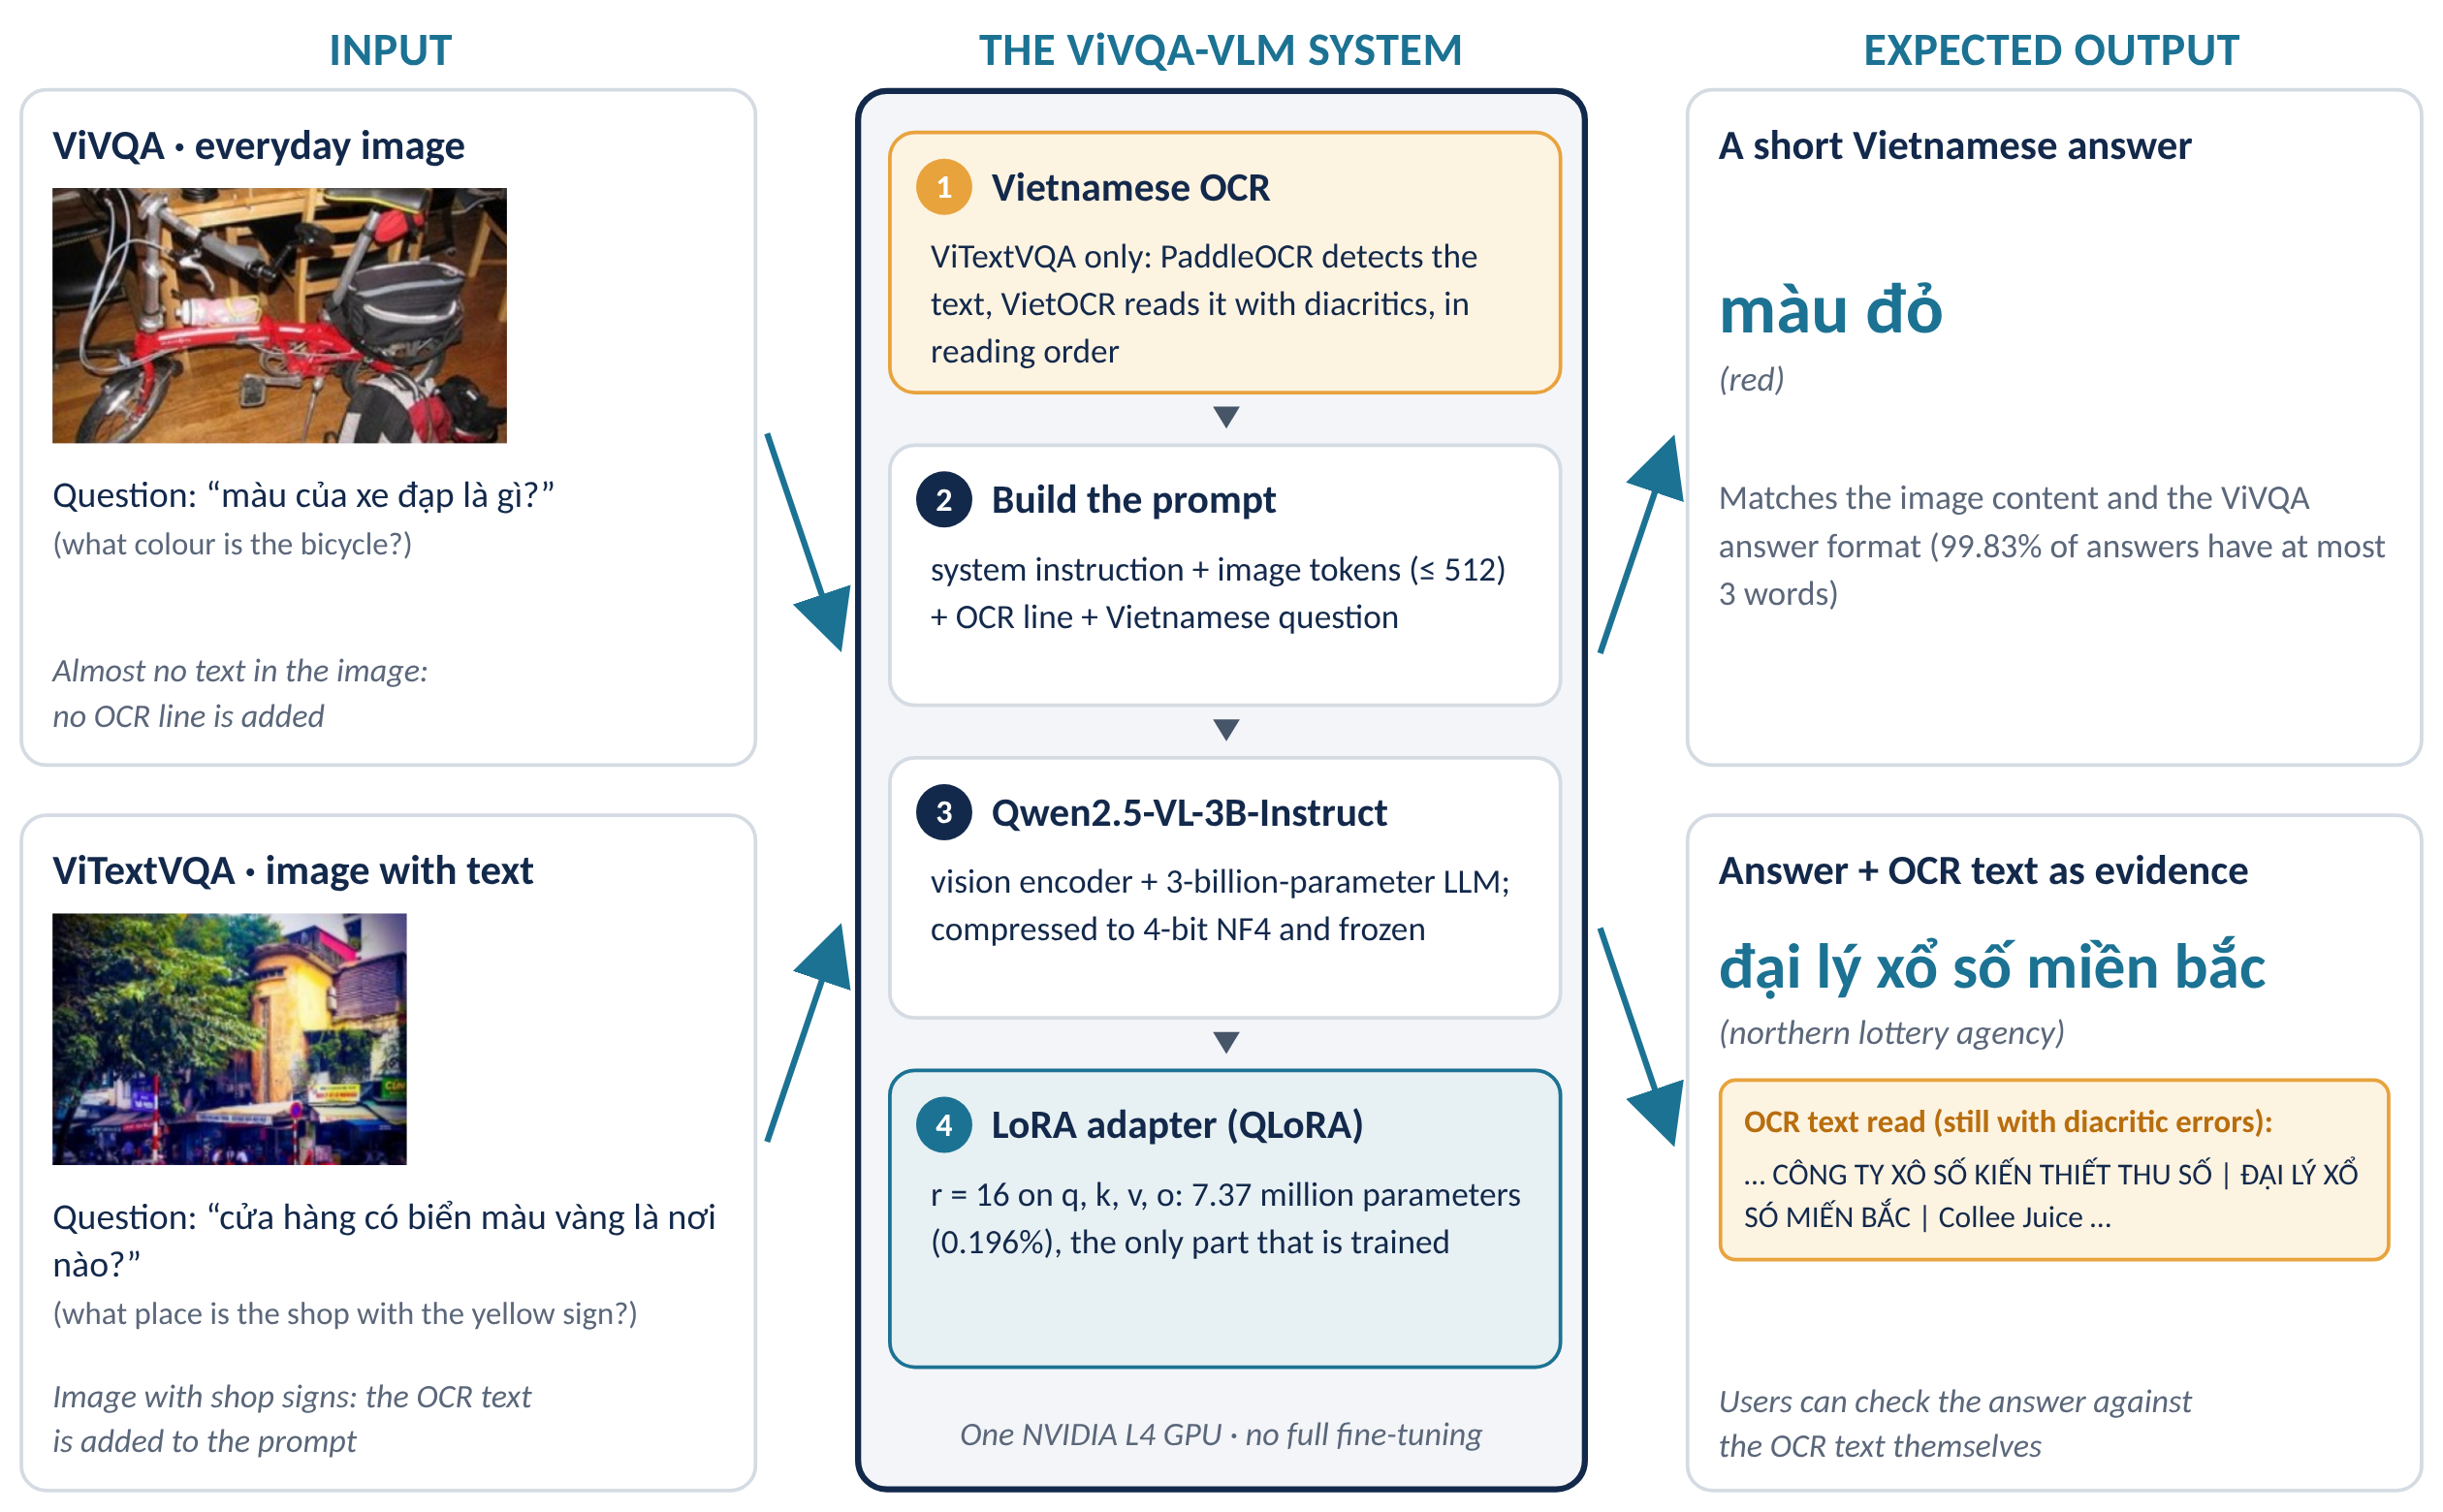
\includegraphics[width=\linewidth]{intro_overview.png}
\caption[Overview of the ViVQA-VLM system]{Overview of the ViVQA-VLM system with one example from each dataset. The
right column shows the gold answers of the two questions; the orange box is the
actual OCR text of ViTextVQA image 16267.jpg, which still contains diacritic
errors. The details of each step are in Chapter~\ref{chap:methods}.}
\label{fig:intro-overview}
\end{figure}

The project is designed as reproducible research, not as a demo application.
Therefore, before any improvement, we reproduce the baseline on a benchmark
with published numbers; every improvement is compared with the baseline under the
same conditions, with statistical tests, ablations, error analysis and
hallucination measurement. The project delivers three things: a model adapted to
Vietnamese, a web prototype verified to give the same answers as the evaluation
pipeline, and this thesis with a reproducibility package (source code, adapters,
configurations, inference scripts and the logs of every run).

%********************************** Section 1.2 ********************************
\section{Background and motivation}
\label{sec:intro-background}

\subsection{Visual question answering and vision-language models}

Visual Question Answering (VQA) asks a system to answer a natural-language question
based on the content of an image~\cite{antol2015vqa}. Unlike image classification or
object detection, VQA requires understanding the image, the meaning of the question
and sometimes the text that appears in the
image~\cite{singh2019textvqa}, \cite{biten2019stvqa}. Early VQA systems combined an image
encoder (a CNN) with a question encoder (an LSTM) and chose the answer from a fixed
set. This works for questions such as ``how many cats are there?'' but not for
questions that require reading: the name of a shop that never appeared in the
training set can never be in the answer set.

Scene-text VQA emerged to address this problem. TextVQA~\cite{singh2019textvqa} and
ST-VQA~\cite{biten2019stvqa} pose questions whose answers must be read from the
text in the image, and M4C~\cite{hu2020m4c} lets the model copy words from the OCR
output into the answer. Recent vision-language models such as
BLIP-2~\cite{li2023blip2}, LLaVA~\cite{liu2023llava},
Florence-2~\cite{xiao2024florence2} and Qwen2.5-VL~\cite{bai2025qwen25vl} change the
approach: an image encoder turns the image into a sequence of tokens, and a large
language model reads this sequence together with the question and generates a
free-form answer. These VLMs can already answer open-ended questions and read text in
images in the zero-shot setting, that is, without additional training for the
specific task.

\subsection{The need to read Vietnamese text in images}

Vietnamese text is everywhere in everyday images: shop signs, price boards, menus,
product labels, road signs and documents. Many of the questions users ask about
these images can only be answered by reading the text correctly: a shop name, an
address, a phone number, a price or an expiry date. For such questions an
approximately correct answer is usually wrong: one wrong digit in a phone number or
one wrong tone mark in a proper name makes the answer useless.

A reliable Vietnamese VQA system can support many applications: assistive
technology that helps visually impaired people read the information around them,
quick lookup of information from photos, and digitisation of content in images.
These applications need a system that not only understands the image but also
reads text with diacritics correctly and answers in natural Vietnamese.

\subsection{Vietnamese and English-centric VLMs}

Most open-source VLMs are pre-trained mainly on English and Chinese data. When they
are used for Vietnamese, we observed four specific problems, labelled V1--V4
and used throughout the thesis:

\begin{description}
  \item[V1, reading text with diacritics.] A tone mark is a tiny stroke;
  misreading one mark changes the meaning (``\vi{BÁNH MÌ}'' read as ``banh mi'').
  The problem is worse when the image has to be downscaled to limit the number of
  image tokens, because a diacritic may then cover only a few pixels. Many OCR tools
  trained for Latin script also drop the diacritics.
  \item[V2, wrong language or wrong format.] The model answers in English, mixes in
  Chinese characters, or answers with a long sentence when the gold answer is only a
  few words. For example, for the question ``\vi{đây là bảo tàng gì?}'' (``what
  museum is this?''), the model answers ``\vi{Bảo tàng Lịch sử Quốc gia.}'' (``The
  National History Museum.'') while the gold answer is ``\vi{lịch sử quốc gia}''
  (``national history''). The answer is semantically correct but does not match the
  gold answer, so it is scored as wrong by Exact Match.
  \item[V3, word order and word boundaries.] Spaces in Vietnamese separate
  syllables, not words; reading the text regions in the wrong order breaks the words
  (``\vi{cửa hàng điện thoại}'', ``phone shop'', becomes ``\vi{cửa điện hàng
  thoại}''). A shop sign usually has several lines of text, so the model also has to
  pick the right phrase and cut it at the right boundaries.
  \item[V4, hallucination.] The answer is fluent but refers to objects or text that
  are not in the image. Because such an answer sounds plausible, users find it hard
  to detect the error, so this problem directly affects the trustworthiness of the
  system.
\end{description}

On Vietnamese data, the gap between machines and humans is still large: on
ViTextVQA~\cite{nguyen2024vitextvqa}, the best published result before this thesis
is 25.48 EM, while humans reach 88.00. Each of the problems V1--V4 is measured
with concrete numbers in Chapter~\ref{chap:results} and summarised in
Chapter~\ref{chap:discussion}.

\subsection{Adapting large models at low cost}

The usual way to bring a pre-trained model to a new task is to fine-tune all of its
parameters. For a VLM with several billion parameters, this requires storing
weights, gradients and optimiser states for every parameter, and therefore several
large GPUs. Parameter-efficient fine-tuning (PEFT) solves this problem by keeping
the base model frozen and training only a small number of added parameters,
for example adapters~\cite{houlsby2019adapter}, \cite{sung2022vladapter} or
LoRA~\cite{hu2022lora}. LoRA adds two low-rank matrices to each linear layer and
trains only these two matrices. QLoRA~\cite{dettmers2023qlora} goes one step
further: the base model is quantised to 4 bits to reduce memory, while the LoRA
adapter is still trained at higher precision.

With QLoRA, adapting a 3-billion-parameter VLM becomes feasible on a single
consumer-grade GPU. The open question is how well this works for Vietnamese, and
what additional information should be given during adaptation so that the model
reads Vietnamese text better. This is the starting point of the thesis.

\subsection{Resource constraints}

Retraining all parameters of a VLM with several billion parameters (full
fine-tuning) requires several large GPUs, which is beyond the means of a student
team. The university did not provide a GPU server for the project, so every
experiment runs on Google Colab, mostly on one NVIDIA L4 GPU with 24~GB. The compute
budget is limited: one QLoRA training run on the whole of ViTextVQA takes about 12
L4 hours, so the number of full training runs is the main constraint on the
experimental plan.

The project therefore makes efficiency an explicit design constraint: it uses only
parameter-efficient fine-tuning (LoRA~\cite{hu2022lora},
QLoRA~\cite{dettmers2023qlora}) and reports training time, inference time and GPU
memory for every result. This constraint also shapes other design choices, for
example the maximum number of image tokens (Chapter~\ref{chap:methods}): the cost of
each choice is measured before it is fixed, instead of choosing the largest
configuration that can run.

%********************************** Section 1.3 ********************************
\section{Problem statement}
\label{sec:intro-problem}

Given an image $I$ and a Vietnamese question $q$, the system generates a Vietnamese
answer $\hat{a} = f(I, q)$. The answer is compared with the gold answer $a$ after
the same text normalisation step. The two datasets place two different demands on
the system:

\begin{itemize}
  \item \textbf{ViVQA}~\cite{tran2021vivqa}: general questions about the image
  (colour, count, objects, position); 99.83\% of the answers have at most 3 words,
  so EM and VQA-Acc are suitable measures.
  \item \textbf{ViTextVQA}~\cite{nguyen2024vitextvqa}: the answer is text read from
  the image, 4.18 words on average; ANLS~\cite{biten2019stvqa} is also used because
  it tolerates small character-level reading errors.
\end{itemize}

In the ViVQA example, the question ``\vi{màu của xe đạp là gì?}'' (``what colour is
the bicycle?'') has the answer ``\vi{màu đỏ}'' (``red''). In the ViTextVQA example,
the question ``\vi{cửa hàng có biển màu vàng là nơi nào?}'' (``what place is the shop
with the yellow sign?'') has the answer ``\vi{đại lý xổ số miền Bắc}'' (``northern
lottery agency''), taken directly from the shop sign
(Fig.~\ref{fig:intro-overview}). The function $f$ must be built by adapting an
open-source VLM using only PEFT, running on one Colab GPU. This general problem is
split into the five sub-problems below.

\subsection{Answering in the right format and the right language}

The first sub-problem is to make the model answer in the answer style of each
dataset: short, in Vietnamese, without explanations. In the zero-shot setting, the
model's answers have 2.9 words on average against 1.6 words for the gold answers on
ViVQA, and 5.4 words against 3.7 words on ViTextVQA; for 18\% of the ViTextVQA
questions the answer contains the gold answer but still fails EM. Unless this format
problem is solved, every other comparison is masked by format errors.

\subsection{Reading Vietnamese text with diacritics}

The second sub-problem is to read text with diacritics correctly. To limit the cost,
each image is represented by at most 512 image tokens; 57.7\% of the ViTextVQA images
reach this cap and must be downscaled, which makes the diacritics even harder to
recognise. Using a separate OCR tool to read the text from the original image is one
way to compensate, but OCR tools can also drop diacritics: PaddleOCR's Latin
recogniser reads ``\vi{Kiểu Thẩm}'' as ``Kiu Thm''. The question is which OCR tool to
use and how to feed its output to the model.

\subsection{Reading order and phrase boundaries}

A ViTextVQA image usually has several text regions: the shop name, a slogan, a phone
number, an address. The third sub-problem is to sort the text regions in the
correct reading order, then pick the right phrase and cut it at the right
boundaries. For example, the gold answer is ``\vi{ủy ban nhân dân quận 2}'' (``District
2 People's Committee'') but the model answers only ``\vi{nhân dân quận 2}'': the text
is read correctly but the boundary is wrong, so the answer is still scored as wrong.

\subsection{Limiting hallucination}

The fourth sub-problem is to make sure that adaptation does not make the model
invent more content. Training the model to give short and confident answers may
unintentionally encourage it to answer even when the image does not contain the
information. Before this thesis there was no POPE-style~\cite{li2023pope}
hallucination benchmark for Vietnamese, so this sub-problem also includes building
the measurement tool.

\subsection{Adaptation and evaluation within limited resources}

The last sub-problem is methodological: adapting the model with less than 1\% of
the parameters trained on one GPU, and evaluating it so that the conclusions can be
trusted. EM is a strict measure under which a semantically correct answer written
differently still counts as wrong, and each full training run costs about 12 GPU
hours, so runs cannot be repeated many times. This requires a fixed evaluation
protocol, paired statistical tests on the same test set, and an experimental design
in which each step changes only one factor.

\paragraph{Factors that make the problem harder.} Besides the five sub-problems
above, the data has several properties that complicate training and evaluation:

\begin{itemize}
  \item some gold answers are wrong: in the manual review of model errors, 12.5\% of
  the errors are due to a wrong gold answer, and 19\% on ViVQA alone;
  \item ViVQA questions were machine-translated from COCO-QA~\cite{ren2015cocoqa}, so
  they are sometimes unnatural, and the dataset has no yes/no questions;
  \item ViVQA has no validation set, and about 46\% of the test questions use images
  that also appear in the training set, which risks overestimating performance;
  \item ViTextVQA has no question-type labels, so errors are hard to break down by
  question type;
  \item some phone photos carry an EXIF rotation flag; if the flag is ignored, OCR
  reads sideways text and produces gibberish.
\end{itemize}

These properties are measured and handled in Chapter~\ref{chap:methods} without
changing the official training and test sets, so that the results remain
comparable with previous work.

%********************************** Section 1.4 ********************************
\section{Research gaps}
\label{sec:intro-gaps}

From the literature review in Chapter~\ref{chap:related}, we identified four
gaps:

\begin{description}
  \item[G1.] English-centric pre-training: zero-shot models answer in English and in
  the wrong format when given Vietnamese questions.
  \item[G2.] Vietnamese VQA is still weak, especially for scene text: the ViTextVQA
  SOTA is 25.48 EM against 88.00 for humans.
  \item[G3.] Adapting VLMs to Vietnamese VQA with PEFT has not been studied: the
  Vietnamese VQA works reviewed either train their own models or use frozen models,
  and none applies LoRA/QLoRA to a large VLM.
  \item[G4.] There is no way to measure hallucination for Vietnamese VQA: no
  POPE-style~\cite{li2023pope} benchmark exists in Vietnamese.
\end{description}

These gaps are related. G1 explains why a strong VLM still performs poorly when used
directly for Vietnamese. G2 shows that the largest gap lies in questions that require
reading text. G3 is a methodological gap: there is no answer yet to the question
``how much can be gained by training only a small adapter on an open VLM, and with
what information should it be trained?''. G4 is an evaluation gap: without measuring
hallucination, it is impossible to know whether adaptation makes the system less
trustworthy.

The thesis focuses on G3 and uses G2 and G4 as places to verify the results. A table
mapping each gap to the evidence in the literature and to how the thesis addresses it
is given in Chapter~\ref{chap:related}.

%********************************** Section 1.5 ********************************
\section{Objectives}
\label{sec:intro-objectives}

The general objective is to adapt an open-source VLM to Vietnamese VQA under a strict
parameter budget and to verify experimentally at least one improvement over a
reproduced baseline. This objective is divided into the specific objectives in
Table~\ref{tab:objectives}, each with a measurable criterion.

\begin{table}[htbp]
\caption{Objectives and completion criteria}
\label{tab:objectives}
\centering
\small
\begin{tabular}{p{0.30\textwidth}p{0.60\textwidth}}
\toprule
\textbf{Objective} & \textbf{Completion criterion} \\
\midrule
Reproduce one baseline correctly &
Re-run Qwen2.5-VL-3B-Instruct on a benchmark with published numbers and reach a small
deviation (TextVQA val: we obtain 79.60 against the published 79.3) \\
Measure the zero-shot baseline on Vietnamese data &
EM, VQA-Acc and ANLS on the full ViVQA and ViTextVQA test sets, with one protocol \\
Adapt with PEFT only &
4-bit QLoRA, fewer than 1\% trainable parameters, running on one Colab GPU \\
Propose and verify $\geq 1$ improvement &
Improvement over the baseline under identical conditions, with a paired statistical
test and ablations \\
Error and hallucination analysis &
Break errors down by question type and error type; measure hallucination with a
POPE-style benchmark for Vietnamese \\
Web prototype &
Upload an image, ask in Vietnamese, receive an answer with the OCR text and a
confidence level; same results as the evaluation pipeline \\
Reproducibility &
Every run records split, seed, hardware, hyperparameters and timing; the package
contains code, adapters, configurations and inference scripts \\
\bottomrule
\end{tabular}
\end{table}

To reach these objectives, we followed a six-step roadmap in which each step
changes only one factor compared with the previous step.

\paragraph{Step 1: Reproduce the baseline.} We re-run Qwen2.5-VL-3B-Instruct on
TextVQA val with the original configuration and compare the result with the number
in the model's technical report. This step checks the whole pipeline for loading the
model, building prompts and scoring before it is used for Vietnamese.

\paragraph{Step 2: Measure zero-shot on Vietnamese data.} With an economical
configuration (4 bits, at most 512 image tokens), we measure the untrained
model on the full test sets of both datasets. This result is the reference point
for all later steps and shows which Vietnamese errors dominate.

\paragraph{Step 3: Adapt with QLoRA.} We train a LoRA adapter on the 4-bit
base model without adding anything to the prompt, to measure the effect of PEFT
alone against zero-shot.

\paragraph{Step 4: OCR-aware QLoRA.} Based on the error analysis of step 3, we
add the Vietnamese OCR text to the prompt during training, not only at inference. The controlled
test is first run on a subset of 8,000 questions, against plain QLoRA on the same
subset; only once the result is clear is it run on the full data.

\paragraph{Step 5: Analysis.} We run ablations for each component, check
stability across three seeds, perform an automatic error analysis checked against a
manual review, and measure hallucination with the Vietnamese POPE benchmark that we
built.

\paragraph{Step 6: Prototype and reproducibility package.} We package the model
as a web prototype, verify that the prototype gives the same answers as the
evaluation pipeline, and prepare a reproducibility package so that others can
re-run every number.

%********************************** Section 1.6 ********************************
\section{Research questions and hypotheses}
\label{sec:intro-rq}

\begin{description}
  \item[RQ1.] How well does zero-shot perform on ViVQA and ViTextVQA, and which
  Vietnamese errors dominate?
  \item[RQ2.] How much does QLoRA improve over zero-shot, without full fine-tuning?
  \item[RQ3.] Does OCR text with diacritics, in the correct reading order, help the
  model read text in images, and does it work together with QLoRA?
  \item[RQ4.] After QLoRA adaptation, does the model invent content more or less
  often?
\end{description}

RQ1 establishes the starting point and the types of errors to fix. RQ2 is the
central question, corresponding to gap G3. RQ3 tests the proposed improvement on the
hardest part of the problem, questions that require reading text (G2). RQ4 checks
the downside of adaptation (G4).

Each hypothesis in Table~\ref{tab:hypotheses} has a quantitative threshold recorded
before the corresponding experiment was run. Because the thresholds were registered in
advance, the verdicts ``supported'', ``partially supported'' or ``not supported''
follow the rules set in advance, not impressions formed after seeing the results.

\begin{table}[htbp]
\caption{Hypotheses and the corresponding research questions}
\label{tab:hypotheses}
\centering
\small
\begin{tabular}{p{0.06\textwidth}p{0.64\textwidth}p{0.18\textwidth}}
\toprule
\textbf{ID} & \textbf{Hypothesis} & \textbf{Answers} \\
\midrule
H1 & QLoRA on Qwen2.5-VL-3B increases EM by at least 5 points over the same model in
the zero-shot setting. & RQ2; V1--V3 \\
H2 & OCR text with diacritics, sorted from top-left to bottom-right and added to the
prompt, increases ANLS by at least 3 points on ViTextVQA; combined with QLoRA it gives
the best result. & RQ3; V1, V3 \\
H3 & A Vietnamese formatting prompt (short answers, with diacritics) increases EM by
at least 3 points and reduces answers in the wrong language or without diacritics. &
RQ1; V2 \\
H4 & QLoRA does not increase the hallucination rate compared with zero-shot. & RQ4;
V4 \\
\bottomrule
\end{tabular}
\end{table}

The results for each research question are reported in Chapter~\ref{chap:results},
their causes are analysed in Chapter~\ref{chap:discussion}, and the combined answers
are given in Chapter~\ref{chap:conclusion}.

%********************************** Section 1.7 ********************************
\section{Contributions}
\label{sec:intro-contrib}

We choose Qwen2.5-VL-3B-Instruct~\cite{bai2025qwen25vl} as the baseline,
reproduce it first, and then adapt it to Vietnamese using QLoRA only. The
3-billion-parameter base model is quantised to 4 bits and kept frozen; we
train only 7.37 million adapter parameters, i.e.\ 0.196\% of all parameters, on one
NVIDIA L4 GPU. The contributions of the thesis are:

\begin{enumerate}
  \item \textbf{OCR-aware QLoRA.} The text read from the image by VietOCR (with
  diacritics, in reading order) is added to the prompt during training, so
  that the adapter learns to use it. On the full ViTextVQA test set (10,028
  questions), this reaches 53.35 EM against 50.26 for plain QLoRA on the same data
  ($+3.09$ EM, McNemar test $p = 6.7\times10^{-21}$), and is far above the best published
  result on the same test set (ViTextBLIP-2, 25.48
  EM~\cite{nguyen2024vitextvqa}).
  \item \textbf{An isolated mechanism.} A $2\times2$ experiment shows that OCR helps
  only when it is used both in training and at inference: adding OCR to the prompt of
  a model that has never seen OCR does not improve the result.
  \item \textbf{Results on general Vietnamese VQA.} On ViVQA, QLoRA raises EM from
  22.09 (zero-shot) to 76.64.
  \item \textbf{A Vietnamese hallucination benchmark.} POPE-vi, with 4,985 yes/no
  questions on 500 images not seen during training.
  \item \textbf{Analysis and a verified prototype.} Ablations for each component,
  automatic and manual error analysis, and a web prototype verified to produce the
  same answers as the official evaluation pipeline.
\end{enumerate}

%********************************** Section 1.8 ********************************
\section{Significance of the work}
\label{sec:intro-significance}

\paragraph{Scientific significance.} The thesis provides a systematic study of PEFT
for VLMs on Vietnamese VQA, with a reproduced baseline, ablations for each component
and paired statistical tests. The main result is not only a higher number but an
isolated mechanism: the benefit of OCR comes from training the model to use OCR, not
from adding OCR to the prompt. We also contribute a Vietnamese POPE benchmark
for hallucination and a quantified analysis of each problem V1--V4. These results can
serve as reference points for future Vietnamese VQA research.

\paragraph{Methodological significance.} Every conclusion in the thesis rests on
decision rules recorded before the run, paired tests on the same test set, and
complete logs (split, seed, GPU, timing). This procedure avoids choosing results
after seeing the numbers and allows others to re-run every number from the public
source code. The thesis also reports results that did not meet expectations, for
example hypothesis H3 was not supported, so that the reader sees the full picture.

\paragraph{Practical significance.} The system reads and answers questions about
Vietnamese shop signs, product labels, price boards, menus and forms. This is a basic
function for assistive technology for visually impaired people and for applications
that look up information from photos. The prototype answers with the OCR text and a
confidence level, so users have a basis to check the answer instead of trusting the
model blindly.

\paragraph{Cost significance.} Because it needs only one GPU and an adapter of
29.5~MB, the approach can be used by research groups, small companies or
organisations with limited resources. One base model can be shared by many tasks,
each needing only a small extra adapter; the thesis also shows that one adapter shared
by both datasets is no worse than a separate adapter per dataset.

\paragraph{Significance for Vietnamese.} Most progress in VLMs is measured on English.
The thesis shows concretely what is lost when these models are used for Vietnamese
(tone marks, format, word order, hallucination) and a low-cost way to recover it. The
approach can be applied to other low-resource languages whose scripts use diacritics.

%********************************** Section 1.9 ********************************
\section{Scope and limitations}
\label{sec:intro-scope}

\subsection{Scope}

\paragraph{Data.} The project uses two public datasets, ViVQA and ViTextVQA, with
their fixed official splits. ViVQA has no validation set, so we hold out
1,200 questions from the training set (seed 42) for model selection; the test set is
unchanged. We do not collect additional training data or use data
augmentation, so that the results are comparable with previous work on the same test
sets.

\paragraph{Model and adaptation.} The project uses exactly one baseline,
Qwen2.5-VL-3B-Instruct. Other VLMs are only used for reference when choosing the
baseline. Adaptation uses 4-bit QLoRA only; the OCR text is an auxiliary input added
to the prompt, not a trained module.

\paragraph{Evaluation.} The main measures are EM, VQA-Acc and ANLS; token-F1 is only a
secondary measure for comparison with previous work. All comparisons use the same
protocol: the same split, seed, inference configuration and the same answer
normalisation step. Besides the main results, the project includes ablations, error
analysis and hallucination measurement.

\paragraph{Prototype.} The prototype is a web application that takes an image and a
Vietnamese question and returns an answer with the OCR text and a confidence level. It
runs on Colab with one GPU or offline on a laptop with a 4~GB GPU. It serves to
illustrate and verify the system, not as a product deployed to many users.

Table~\ref{tab:scope} summarises what is in and out of scope.

\begin{table}[htbp]
\caption{In scope and out of scope}
\label{tab:scope}
\centering
\small
\begin{tabular}{p{0.45\textwidth}p{0.45\textwidth}}
\toprule
\textbf{In scope} & \textbf{Out of scope} \\
\midrule
Two datasets, ViVQA and ViTextVQA, with fixed splits &
Building a new training dataset or data augmentation \\
One baseline, Qwen2.5-VL-3B-Instruct; other VLMs for reference only &
Comparing several backbones as main baselines \\
Adaptation with PEFT only (4-bit QLoRA); OCR text as auxiliary input &
Full fine-tuning; training a VLM from scratch \\
Metrics EM, VQA-Acc, ANLS (token-F1 as a secondary measure); ablations, error
analysis, hallucination & Retrieval-augmented VQA with external knowledge \\
Web prototype on one Colab GPU or offline on a laptop with a 4~GB GPU &
Large-scale product deployment, mobile applications \\
\bottomrule
\end{tabular}
\end{table}

\subsection{Limitations}

\paragraph{Model limitations.} The results are bounded by a 3-billion-parameter base
model in 4-bit form. Quantisation reduces accuracy compared with the original
configuration, and a larger model may give different results. The thesis does not
claim that the results hold for other backbones.

\paragraph{OCR limitations.} The proposed method depends on the quality of the OCR.
When the OCR line does not contain the correct answer, the model can hardly answer
correctly; blurry images, small text or decorative fonts can still make OCR misread
the diacritics or produce gibberish.

\paragraph{Data limitations.} Some gold answers are wrong, ViVQA questions are
machine-translated, and ViVQA has no yes/no questions. We measure these issues
and report them separately, but do not modify the official test sets.

\paragraph{Evaluation limitations.} EM is strict towards answers that are correct in
meaning but written differently, so we add ANLS and a manual review. The
comparison with previous work also depends on answer normalisation steps that those
works do not fully publish; we additionally report token-F1 to reduce the
effect of this issue.

\paragraph{Statistical limitations.} All main experiments run with one seed; only the
OCR comparison is additionally checked with three seeds on the 8,000-question
subset. The full model B3-full has only one seed, because each training run costs
about 12.75 GPU hours.

\paragraph{Prototype limitations.} The prototype's confidence is not well calibrated,
so the interface shows only High, Medium and Low levels instead of a percentage. The
prototype runs in a Colab session or on a single laptop, so it does not have the
availability of a real service. On the laptop, OCR runs on the CPU and takes several
seconds for each new image.

These limitations are analysed again in Chapter~\ref{chap:discussion} and
Chapter~\ref{chap:conclusion}.

\subsection{Out of scope}

The following are outside the scope of the thesis:

\begin{itemize}
  \item full fine-tuning or training a VLM from scratch;
  \item building a new training dataset, additional labelling or data augmentation;
  \item retraining or fine-tuning the OCR models;
  \item retrieval-augmented VQA with knowledge sources outside the image;
  \item comparing several backbones as several main baselines;
  \item large-scale product deployment, mobile applications or long-running online
  services;
  \item questions about videos or several images at once.
\end{itemize}

\paragraph{Assumptions.} We make three assumptions. First, the official splits of the two
datasets represent the actual question distribution of each dataset. Second, the gold
answers are correct for most questions; the share of wrong gold answers is measured and
reported separately in Chapter~\ref{chap:results}. Third, the L4 GPU on Colab gives
stable results across sessions when the seed and the configuration are fixed.

%********************************** Section 1.10 *******************************
\section{Team organisation}
\label{sec:intro-team}

\subsection{Structure and roles}

The team has four students, each in charge of one technical area as defined in the
project proposal.

Pham Le Huy Hoang (SE182670) is the team leader and is in charge of PEFT / Training.
Besides training the QLoRA models, running the LoRA configuration ablations and
building the shared adapter, Hoang coordinates the schedule, integrates the results
of the different areas and reviews cross-area results.

Ho Dac Toan (SE183249) is in charge of VLM / Baseline: studying the Qwen2.5-VL
architecture, reproducing the zero-shot baseline and comparing it with the published
numbers.

Tran Quoc Huan (SE193642) is in charge of Dataset / OCR: obtaining the data from the
official sources, fixing the splits, checking for leakage between training and test,
and building the OCR cache with PaddleOCR and VietOCR.

Van Quang Truong (SE182458) is in charge of Evaluation / Deployment: implementing the
metrics and statistical tests, measuring hallucination, and building the prototype and
the demo video.

The detailed assignment table, with each member's main source-code directories, is in
Appendix~\ref{appendix:pm}.

\subsection{Communication plan}

The team works with the supervisors at the department's milestones and whenever a
major decision needs confirmation, for example fixing the Qwen2.5-VL-3B baseline on
7 October 2026. After each review meeting, the team fills in the feedback checklist,
emails it to the supervisors and the reviewers, and uploads it to the shared folder.

Within the team, each working week has a README and a Team Report in the
\path{docs/Wxx/} directory of the repository, recording what was done, the results,
the decisions and what was postponed. Source code, small logs and documents are
managed on GitHub; images, adapters, the OCR cache and the demo video are stored on
Google Drive. Decisions that affect the main results are recorded before the run and
confirmed by the supervisors when needed.

%********************************** Section 1.11 *******************************
\section{Project management approach}
\label{sec:intro-pm}

Because this is a research project, the plan revolves around experiments: every
conclusion in Chapter~\ref{chap:results} must be traceable to a run with a log, a seed
and a fixed configuration. This section summarises how the team organised the work;
Appendix~\ref{appendix:pm} presents the full work breakdown, schedule, risks and
quality management.

\subsection{Phases}

The project is divided into five phases following the 15-week frame of the proposal:

\paragraph{Phase 1: Orientation and planning (W01--W03).} The team reads papers in the
four areas, builds a literature matrix, analyses the two datasets, identifies the
research gaps, research questions and hypotheses, and presents them at Review~1.

\paragraph{Phase 2: Data and baseline (W04--W07).} The team obtains the data from the
official sources, fixes the Qwen2.5-VL-3B-Instruct baseline, measures zero-shot,
reproduces the published number on TextVQA and fixes the inference configuration
based on measurements (number of image tokens, data type).

\paragraph{Phase 3: Adaptation and improvement (W07--W10).} The team trains plain
QLoRA, analyses the errors, proposes OCR-aware QLoRA, verifies it on the
8,000-question subset, checks it across three seeds and with the $2\times2$ table, and
then runs it on the full data.

\paragraph{Phase 4: Evaluation and analysis (W10--W12).} The team builds the full
evaluation table, runs the LoRA configuration ablations, tries a shared adapter,
analyses the errors and measures hallucination with the Vietnamese POPE benchmark.

\paragraph{Phase 5: Prototype, packaging and thesis (W13--W15).} The team builds the web
prototype, verifies that it matches the evaluation pipeline, records the demo video,
and prepares the reproducibility package, the defence slides and the thesis.

\subsection{Integrating the components}

The components of the system are connected through a few fixed shared points. A
single prompt-building function is used for training, evaluation and the prototype,
so the prompt never differs between stages. OCR is run once and cached with a hash;
training and evaluation only read the cache. The list of official models is generated
automatically from the logs, and the prototype is checked against pre-set rules to
make sure it gives the same answers as the evaluation pipeline.

\subsection{Quality and risk management}

The quality of the project is first of all the reliability of its numbers. The team
commits the decision rule of each main test to Git before running it, uses paired
tests for every comparison, recomputes the result tables directly from the original
prediction files instead of copying them by hand, and records SHA-256 hashes for the
adapters, the OCR cache and the data files.

As for risks, the initial plan listed eight risks. Those that actually occurred were:
no GPU server at the university, fp16 corrupting the answers on the T4 GPU, data
initially taken from the wrong source, about 12 hours per full training run, and
images with an EXIF rotation flag corrupting the OCR cache. How each risk was handled
is described in Appendix~\ref{appendix:pm}.

\subsection{Progress tracking}

The team works in weekly cycles: plan, record the rules in advance, run the
experiments, re-check the numbers, and close the week with a README and a Team
Report. Progress is checked against the department's milestones: Review~1, Review~2,
the department committee and the university committee. When a decision changes the
plan, for example changing the baseline or moving to Colab, the decision and its
reason are recorded in the weekly report.

%********************************** Section 1.12 *******************************
\section{Thesis outline}
\label{sec:intro-outline}

Chapter~\ref{chap:related} reviews VQA, vision-language models, parameter-efficient
fine-tuning and Vietnamese VQA research. Chapter~\ref{chap:methods} presents the data,
the baseline, the OCR-aware QLoRA method and the evaluation protocol.
Chapter~\ref{chap:results} reports the main results and the ablations.
Chapter~\ref{chap:discussion} discusses the error analysis, hallucination and
limitations. Chapter~\ref{chap:conclusion} concludes. Appendix~\ref{appendix:pm}
presents the project management plan, and Appendix~\ref{appendix:repro} describes the
reproducibility package.
